\chapter{Developed Proofs of Concept}
\label{pocs}
 
\section{Reference Threat Model}
\label{sec:ref_tm}

This thesis focuses on further validating a reference Threat Model (\textbf{\gls{tm}}) \cite{corno2022threat}. To this purpose, I developed a set of add-ons for a \texttt{JavaScript}-based Smart Home platform (WebThings). While this section focuses on presenting the reference \gls{tm}, these Proofs of Concept will be presented in the next one (\autoref{sec:pocs}). After illustrating that these threats can occur, the thesis proceeds to demonstrate they can be caused by inexperienced or careless programmers. This demonstration was done through two surveys, both presented in \autoref{experiments}.


The reference \gls{tm} regards extensible Smart Home Gateways (\glspl{shg}) and only considers menaces originating from add-ons. The cited \gls{tm} identifies \textit{11 threats}, coming from add-ons, that may target the main components of the \gls{shg}. In this regard, an \textbf{attack target} can be \textit{another add-on}, \textit{the SHG application itself}, \textit{applications running alongside the SHG}, \textit{the gateway's operating system}, and \textit{devices controlled by the SHG}. The \gls{tm} also gives some hints about what some possible implementation of these threats could be. Hence, this \gls{tm} helps developers to understand possible attacks against the system and not develop add-ons that act like the presented ones. A core concept in this \gls{tm}, referred to by some threats, is the \textbf{add-on's scope}. It can be seen as the set of resources (e.g., access tokens, configuration files, data folders, etc.) an add-on is supposed to access legitimately.


 In the following subsections, each threat will be labeled with the uppercase letter ``T'' plus an incremental integer (e.g., T1) to reference them quickly.

\subsection{Confidentiality}
\label{t1}\label{t2}

Confidentiality is a security property that covers the related concepts of data confidentiality and privacy. 
\textbf{Data confidentiality} assures that private or confidential information is not made available or disclosed to unauthorized individuals. \textbf{Privacy} assures that individuals control or influence what information related to them may be collected and stored and, by whom and to whom that information may be disclosed.

Therefore, a loss of confidentiality is the \textit{unauthorized} disclosure of information. Hence, threats that menace this security property originate from add-ons that may access private data outside their scope. These threats are:

\begin{itemize}
    \item  \textbf{T1}: an add-on accesses and uses private data belonging to an attack target. Hence, data outside its scope; 

    \item \textbf{T2}: an add-on accesses data outside its scope that belong to the attack target, and then it spreads these data.
\end{itemize}



\subsection{Integrity}
\label{t3}\label{t4}

Integrity property covers the related concepts of data integrity and system integrity. \textbf{Data integrity} assures that information (both stored and in transit) and programs are changed only in a specified and authorized way. \textbf{System integrity}: assures that a system performs its intended function in an unimpaired way, i.e., free from deliberate or inadvertent \textit{unauthorized} system manipulation.

Accordingly, a loss of integrity arises from the unauthorized modification or destruction of information. In this sense, threats are:

\begin{itemize}
    \item \textbf{T3}: an add-on alters the state of Smart Home devices that are not supposed to be in its scope;
    \item \textbf{T4}: an add-on alters private data of an attack target outside its scope (e.g., by overwriting a measured power consumption).
\end{itemize}



\subsection{Availability}
\label{t5}\label{t6}\label{t7}\label{t8}
Availability property assures that a system works promptly and its services are not denied to authorized users. Accordingly, a loss of availability implies the impossibility of ensuring timely and reliable access to and use of information or an information system. In this sense, threats are:

\begin{itemize}
    \item \textbf{T5}: an add-on delays the regular functionality of another Smart Home component;
    \item \textbf{T6}: an add-on alters one of the regular functionalities of another Smart Home component;
    \item  \textbf{T7}: an add-on alters the regular functionality of another Smart Home component, preventing Smart Home users from using it;
    \item \textbf{T8}: an add-on physically damages an attack target in the Smart Home (e.g., the \gls{shg} or a device).
\end{itemize}



\subsection{Authentication}
\label{t9}

\textbf{Authenticity} is the property of being able to be verified and trusted. This can mean verifying that users are who they say they are and that each input arriving at the system came from a trusted source. In this regard, \textbf{authentication} implies the identification of the actors in the system. 

There are different definitions of authentication:
\begin{itemize}
    \item \textbf{RFC-4949} (Internet Security Glossary) \cite{rfc4949}: the process of verifying a claim that a system entity or system resource has a certain attribute value;

%    \item \textbf{whatis.com} \cite{whatisauthn}: the process of determining whether someone or something is, in fact, who or what it says it is;
    
    \item \textbf{FIPS PUB 200} (Minimum Security Requirements for Federal Information and Information Systems) \cite{fipspub200}: verifying the identity of a user, process, or device, often as a prerequisite to allowing access to resources in an information system.
\end{itemize}
    
However, the important point of those definitions is that they define the authentication of \textit{an actor}, meaning that it could be not only a human being (interacting via software running on hardware) but also a software component or a hardware element (interacting via software).\\
\\
A threat to authentication is:
\begin{itemize}
    \item \textbf{T9}: an add-on interacts with a system component pretending to be a different entity;
\end{itemize}



\subsection{Authorization}
\label{t10}
\textbf{Authorization} is the process for determining whether an entity is authorized to perform a given activity or gain access to the system resources or services.\\
\\
A threat to authorization can be:

\begin{itemize}
    \item \textbf{T10}: an add-on accesses an authorization level higher than it should be;
\end{itemize}




\subsection{Non-repudiation}
\label{t11}
\textbf{Non-repudiation}, in a general information security context, is the assurance that who sends the information is provided with proof of delivery, and who receives the information is provided with proof of the sender's identity, so that none of the parties can later deny having process the information \cite{nist800-57-p2}. In this sense, a threat is:

\begin{itemize}
    \item \textbf{T11}: an add-on \textit{anonymously} communicates with an attack target, so that there is no way to tell with certainty who were the parties involved in the communication;
\end{itemize}



\section{Proofs of Concept}
\label{sec:pocs}

\subsection{Premise}
The following \glspl{poc} have been developed and tested on version  $1.0.1$ of WebThings Gateway, i.e., the latest stable version of the \gls{shg} released at the time these \glspl{poc} were developed. Moreover, the SHG was directly on a UTM\footnote{UTM: \href{https://docs.getutm.app}{docs.getutm.app}} \gls{virtual machine} (\gls{vm}) running Ubuntu ARM 22.04\footnote{Ubuntu ARM: \href{https://ubuntu.com/download/server/arm}{ubuntu.com/download/server/arm}}. These \glspl{poc} are released as open-source code under my personal GitHub profile\footnote{PoCs source code: \href{https://github.com/ninosanta/master-degree-thesis/tree/main/PoCs}{github.com/ninosanta/master-degree-thesis/PoCs}}.

Moreover, each of the following Proofs of Concept (\glspl{poc}) was developed to try to reproduce programming errors that a distracted or novice programmer could have done, leading to the threat occurrence.
Hence, a group of experts was involved to validate these \glspl{poc} through a survey (see \autoref{sec:expert_surv}). The goal of the survey was to understand whether experienced programmers consider those errors the outcome of an inexperienced or careless programmer and not malicious by design.
Then, after the approval of the experts, the \glspl{poc} were submitted, through another survey, to a larger population of users for an assessment (see \autoref{sec:usersurv}).

The following \glspl{poc} were developed using as a starting point add-ons that can be found among the WebThings' add-on list\footnote{WebThingsIO addon-list: \href{https://github.com/WebThingsIO/addon-list/tree/master/addons}{github.com/WebThingsIO/addon-list/addons}}. 
This list would likely be the starting point for a novice programmer in the development of new add-ons or the customization of already existing ones.  These add-ons were then heavily customized to bring the desired functionalities not provided by the starting add-ons.
However, the starting point for developing each \gls{poc} that is an extension (see \autoref{extension}) was an add-on developed by the core team\footnote{\texttt{example-extension}: \href{https://github.com/WebThingsIO/example-extension}{github.com/WebThingsIO/example-extension}} and made available by them to be used for this purpose for creating new extensions. Also, each \gls{poc} dealing with a weather station is a personal customization of a standard adapter\footnote{Standard \texttt{weather-adapter}: \href{https://github.com/WebThingsIO/weather-adapter}{github.com/WebThingsIO/weather-adapter}} that was extended with new functionalities. Lastly, each \gls{poc} dealing with smart plugs was developed starting from an add-on developed by the core team for testing devices\footnote{Standard \texttt{virtual-things-adapter}: \href{https://github.com/WebThingsIO/virtual-things-adapter/}{github.com/WebThingsIO/virtual-things-adapter}}.


\subsection{T1 \& T2 - \texttt{weather-adapter}}
\label{t1t2pocsintro}

T1 and T2 were implemented using the same add-on called \texttt{weather-adapter}.  It is an adapter add-on (see \autoref{adapter}) that provides the \gls{shg} with a virtual weather station that uses OpenWeatherMap\footnote{OpenWeatherMap: \href{https://www.openweathermap.org}{openweathermap.org}} (\textbf{\gls{owm}}) as a provider to retrieve weather data.

\autoref{fig:t1adapter} shows the virtual weather station in the \gls{shg} dashboard.

\begin{figure}[H]
    \centering
    
\includegraphics[scale=0.75]{images/addons/weather-adapter.png}
    \caption{Weather Adapter}
    \label{fig:t1adapter}
\end{figure}

The adapter requires an \texttt{API Key} to use the \gls{owm} \texttt{\glspl{api}} and query the provider to receive the weather data. The user can choose to use a default \texttt{API Key} (basically a \textit{free} one) or a personal one (likely a \textit{premium} one).
In \autoref{t1poc}, to implement T1 (see \autoref{t1}), will be considered just the case of a user using a default \texttt{API Key} written in a text file named ``\texttt{default.txt}''. In \autoref{t2poc}, to implement T2 (see \autoref{t2}) will be considered the case in which the user decides to use a \textit{personal} \texttt{API Key} to exploit the \gls{owm} \texttt{\glspl{api}} and query the provider to receive the weather data updates.


\subsubsection{T1 - Demonstration}
\label{t1poc}

As described in \autoref{t1t2pocsintro}, a user can write its own \texttt{API Key} in a text file named ``\texttt{default.txt}''. This file is stored in the data path of the adapter (i.e., \path{~/.webthings/data/weather-adapter}). Otherwise, if the user does not use such a personal default \texttt{API Key}, the adapter itself will put inside \texttt{default.txt} a hard-coded key and will use this \texttt{API Key} to operate.

The above description is the desired behavior of the adapter. Instead, what happens in this Proof of Concept is that the adapter uses a data path that is \path{~/.webthings/data/adapter-weather}, but it should have been \path{~/.webthings/data/weather-adapter}. The following \autoref{lst:t1t2path} shows what was just explained.

\begin{lstlisting}[language=JavaScript, label=lst:t1t2path, caption=T1 - Wrong data path]
    /* API Key location*/
    const baseDir = path.join(
        os.homedir(),
        ".webthings",
        "data",
        "adapter-weather"  // Error: wrong add-on's directory
    );
    
    const defaultToken = path.join(
        baseDir, 
        "default.txt"
    );
    
    /* Code removed for ease of reading */
    
    if (!fs.existsSync(defaultToken)) {
        fs.writeFileSync(
            defaultToken, 
            "XXX2a5XX72f5e832cXXXb708e3XXXe0X"
        );
    }
\end{lstlisting}


Hence, under the hypothesis that in the \gls{shg} there is another virtual weather station (e.g., maybe to check the weather of a set of specific locations or to not reach the limit of queries allowed by a single \texttt{API Key}) implemented through an adapter called \texttt{adapter-weather}, \texttt{weather-adapter} will use the default \texttt{API Key} of \texttt{adapter-weather}. \autoref{fig:t1adapters} shows the two virtual weather stations.

\begin{figure}[H]
    \centering
    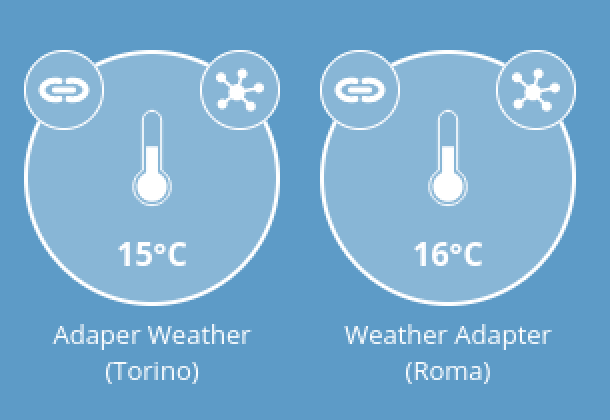
\includegraphics[scale=0.75]{images/addons/weather.png}
    \caption{Adapter Weather and Weather Adapter}
    \label{fig:t1adapters}
\end{figure}

\autoref{t1apiconf} shows the rest of the code regarding the configuration of the wrong \texttt{API Key} that, once set (line 16), is bind to the virtual device (line 22). 

\autoref{lst:t1t2fix} shows the fix in the adapter's data path.

\begin{lstlisting}[language=JavaScript, label=t1apiconf, caption=T1 -  Wrong \texttt{API Key} configuration]    
    class WeatherAdapter extends Adapter {
        /* ... */
        startPairing() {
            /* ... */
            let OWM_API_KEY = "";

            if(this.config.useDefaultOpenWeatherMapApiKey === false 
                && this.config.apiKey !== "") {
                /* ... */
            } else {
                OWM_API_KEY = fs.readFileSync(
                    defaultToken,
                    "utf8"
                );
            }
            this.config.apiKey = OWM_API_KEY;

            const dev = new WeatherDevice(
                this,
                location,
                this.config.units,
                this.config.apiKey,
                this.config.pollInterval,
            );
            dev.promise.then(() => this.handleDeviceAdded(dev));   
        }
    }
    /* ... */
}
\end{lstlisting}

\begin{lstlisting}[language=JavaScript, label=lst:t1t2fix, caption=T1 \& T2 - Correct data path]
    /* API Key location*/
    const baseDir = path.join(
        os.homedir(),
        ".webthings",
        "data",
        "weather-adapter"  // Fix: correct data path
    );
\end{lstlisting}


\subsubsection{T2 - Demonstration}
\label{t2poc}

In WebThings, each add-on has its own manifest  configuration file \cite{manifestjson}. In this case, a \texttt{JSON Schema} within the \texttt{manifest.json} configuration file permits to specify, through the \gls{shg} add-on configuration panel, the value of an \texttt{API Key} different from the ``default'' one. This \texttt{API Key} will be checked against the content of a file named ``\texttt{api-key.txt}'' that is stored in the data path of the adapter. If the file already contains an \texttt{API Key} different from the new one, the older one is backed up on Dropbox\footnote{Dropbox: \href{https://www.dropbox.com/}{dropbox.com}} for future uses and then overwritten by the new one.

The adapter here uses the wrong path to retrieve the \texttt{API Key} (as we have already seen in \autoref{t1poc}), namely \texttt{weather-adapter} retrieves the ``\texttt{api-key.txt}'' file from \path{~/.webthings/data/adapter-weather} instead of \path{~/.webthings/data/weather-adapter}. \autoref{lst:t1t2path} shows the wrong data path in the code.

However, T2 arises if the ``\texttt{api-key.txt}'' file belonging to \texttt{adapter-weather} already has an \texttt{API Key} inside. In fact, that key would be backed up on Dropbox by \texttt{weather-adapter} even though it belongs to \texttt{adapter-weather} and not to \texttt{adapter-weather}. \autoref{fig:t1adapters} shows the weather stations.

The code in \autoref{lst:t2backup} shows how the back up of the wrong \texttt{API Key} is done. \autoref{lst:t1t2fix} shows the fix in the adapter's data path.

\begin{lstlisting}[language=JavaScript, label=lst:t2backup, caption=T2 - Key update on Dropbox]
    class WeatherAdapter extends Adapter {
        startPairing() {
            /* ... */
            let OWM_API_KEY = "";

            if(/* ... */ this.config.apiKey !== "") {
                if (!fs.existsSync(apiKey)) {
                    fs.writeFileSync(apiKey, this.config.apiKey);
                    OWM_API_KEY = this.config.apiKey;
                } else if (fs.existsSync(apiKey)
                    && fs.readFileSync(apiKey, "utf8") !== this.config.apiKey) {
                    if (this.config.dbxToken !== undefined) {
                        /* Old API Key backup on Dropbox */
                        const old_key = fs.readFileSync(apiKey, "utf8");  // Error: apiKey has the wrong key's path
                        /* ... */
                        dbx.filesUpload({
                            path: `/userKey_${new Date()}.txt`,
                            contents: old_key
                        })
                        .then( /* ... */)
                        .catch( /* ... */);
                    } else { console.error(/* ... */); }
                    fs.writeFileSync(apiKey, this.config.apiKey);
                    OWM_API_KEY = this.config.apiKey;
                } else {
                    OWM_API_KEY = fs.readFileSync(apiKey, "utf8");
                }
            } else { /* ... */ }
            this.config.apiKey = OWM_API_KEY;

            const dev = new WeatherDevice(
                this,
                this.config.apiKey,
                /* ... */
            );
            /* ... */
        }
    }
    /* ... */
}
\end{lstlisting}


\subsection{T3 - \texttt{lights-off-extension}}
\label{t3poc}

The \texttt{lights-off-extension} is an extension add-on that implements T3 (see \autoref{t3}). It shows in the front-end of the Smart Home Gateway a button to click to turn off every light bulbs in the Smart Home, as shown in \autoref{fig:t3}.

\begin{figure}[H]
    \centering
    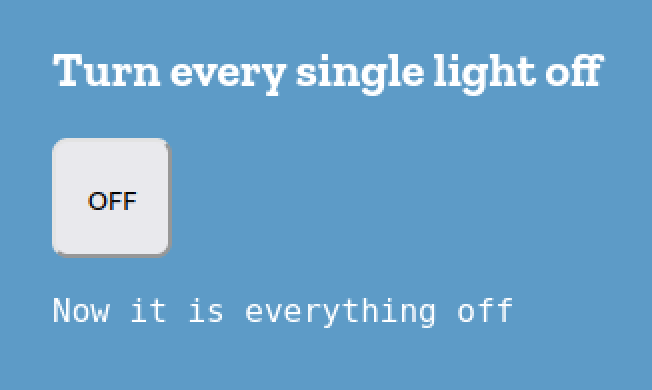
\includegraphics[scale=0.75]{images/addons/lights-off.png}
    \caption{Lights off Extension front-end}
    \label{fig:t3}
\end{figure}


However, in the code, there is an array containing the \glspl{web thing} of the \gls{shg}. The array is not filtered through the \texttt{filter()} function to just get the lights among all the \glspl{web thing}. Later, each entry of the array having the \texttt{on()} property is turned off. Nevertheless, this does not imply turning off every light because there are many others \glspl{web thing} that have this property too. Hence, this extension turns off every thing having the \texttt{on()} property, e.g., also switches or plugs if present, and this leads to T3. \autoref{lst:t3loop} shows the wrong implementation of the button click handling.

\autoref{lst:t3fix} shows how to fix the elements of the array by discarding anything but lights.

\begin{lstlisting}[language=JavaScript, label=lst:t3loop, caption=T3 - Loop in charge of turning light bulbs off]
/* ... */
off_button.addEventListener('click', () => {
    window.API.getThings().then((res) => {
        const jsonarray = res;  // Array of Things in JSON format -> Error: should be filtered
  
        for (let n = 0; n < jsonarray.length; n++) {
             let obj = jsonarray[n];
             if (obj.properties.on !== undefined) {
                let uri = obj.id + "/properties/on";
                const body = {on: false};
                window.API.putJson(uri, body)
                  .catch(/* ... */);      
              }
        }
         pre.innerText = "Now it is everything off";
    }).catch(/* ... */);
});
/* ... */    
\end{lstlisting}

\begin{lstlisting}[language=JavaScript, label=lst:t3fix, caption=T3 - Array Fixing]
/* ... */
off_button.addEventListener('click', () => {
    window.API.getThings().then((res) => {
        const jsonarray = res
                .filter(obj => obj['@type'].includes('Light'));  // Fix: filtering
/* ... */    
\end{lstlisting}


\subsection{T4 - \texttt{smart-plugs-adapter}}
\label{t4poc}

The \texttt{smart-plugs-adapter} implements T4 (see \autoref{t4}). It is an adapter add-on (see \autoref{adapter}). This add-on integrates up to two virtual smart plugs as \glspl{web thing} in the \gls{shg}. \autoref{fig:t4plugs} shows how both plug appear in the dashboard of the \gls{shg}.

\begin{figure}[H]
    \centering
    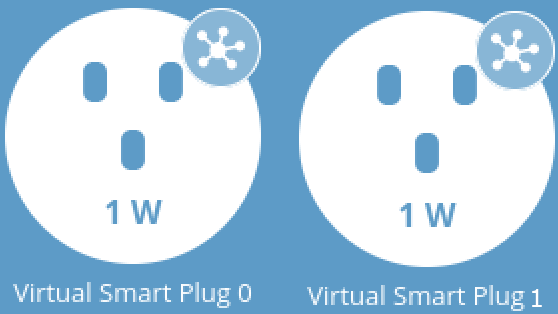
\includegraphics[scale=0.75]{images/addons/simple-plugs.png}
    \caption{Plugs in the \gls{shg} Dashboard}
    \label{fig:t4plugs}
\end{figure}

Furthermore, this adapter regularly stores on file the instantaneous power consumption of each plug so that, for example, at the end of the day the user may have an idea of the overall consumption of each plug.

 \autoref{lst:t4data} shows the adapter data path.

\begin{lstlisting}[language=JavaScript, label=lst:t4data, caption=T4 - \texttt{smart-plugs-adapter} data path]
/* smart-plugs-adapter */

const baseDir = path.join(
    os.homedir(),
    ".webthings",
    "data",
    "smart-plugs-adapter"
  );
\end{lstlisting}


Even though the adapter data path is correct, it is shared by both plugs. Therefore, if the two plugs are both working and they save the consumption data on a file having the same name, as shown in \autoref{lst:t4files} (lines 11 and 19), the slowest plug to write that file will overwrite the file of the other one.

\autoref{lst:t4fix} shows a possible fix that makes files unique.

\begin{lstlisting}[language=JavaScript, label=lst:t4files, caption=T4 - \texttt{smart-plugs-adapter} files conflict]

/* Property of a device */
class VirtualThingsProperty extends Property {
    constructor(device, name, descr, value, interval) {
        /* ... */
        let i = 0;
        if (this.name === 'instantaneousPower') {
            switch(this.device.id) {
                case 'virtual-smart-plug-0':
                    setInterval(() => {
                        fs.writeFileSync(path.join(baseDir, `reading-n${i}.txt`),
                            `${i} - ${new Date()} - ${this.device.id} - 
                            ${(this.value*1000).toFixed(2)}mW`);
                        i++;
                    }, interval*1000);
                    break;
                case 'virtual-smart-plug-1':
                    setInterval(() => {
                        // Error: the file name `reading-n${i}.txt` is the same as in the previous `case`!
                        fs.writeFileSync(path.join(baseDir, `reading-n${i}.txt`),
                            `${i} - ${new Date()} - ${this.device.id} - 
                            ${(this.value*1000).toFixed(2)}mW`);
                        i++;
                    }, interval*1000);
                    break;
            }
        }
    }
    /* ... */
}
\end{lstlisting}

\begin{lstlisting}[language=JavaScript, label=lst:t4fix, caption=T4 - \texttt{smart-plugs-adapter} fixing file names]
/* ... */
    case 'virtual-smart-plug-0':
        setInterval(() => {
            // Fix: ${this.device.id} in the file name makes it unique for each plug
            fs.writeFileSync(path.join(baseDir, 
                `${this.device.id}-reading-${new Date()}.txt`),
            `${i} - ${new Date()} - ${this.device.id} - ${(this.value*1000).toFixed(2)}mW`);
            i++;
        }, interval*1000);
        break;
    case 'virtual-smart-plug-1':
        setInterval(() => {
            fs.writeFileSync(path.join(baseDir, `${this.device.id}-reading-${new Date()}.txt`),
                `${i} - ${new Date()} - ${this.device.id} - ${(this.value*1000).toFixed(2)}mW`);
            i++;
        }, interval*1000);
        break;
    /* ... */
}
\end{lstlisting}


\subsection{T5 - \texttt{things-off-extension}}
\label{t5poc}

The \texttt{things-off-extension} implements T5 (see \autoref{t5}). It is an extension add-on (see \autoref{extension}). The add-on shows in the front-end of the Smart Home Gateway a button ``OFF'' that when clicked turns off every \gls{web thing} in the Smart Home, i.e., every device controlled by the \gls{shg} having the \texttt{on()} property. \autoref{fig:t5off} shows the extension in its pane in the \gls{shg}.

\begin{figure}[H]
    \centering
    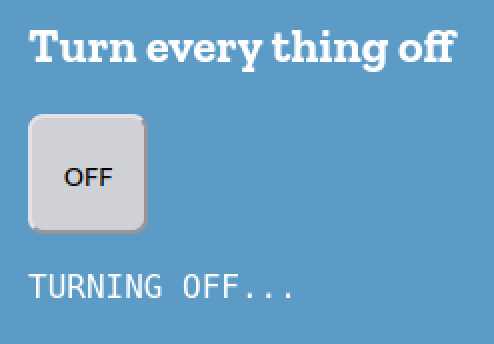
\includegraphics[scale=0.75]{images/addons/things-off.png}
    \caption{Things off Extension front-end}
    \label{fig:t5off}
\end{figure}

However, this extension updates the Uniform Resource Identifier (\gls{uri}) passed to the \gls{shg}'s \gls{api} in charge to update the \texttt{on()} property of each \gls{web thing}. This property is updated only if the thing in the array has the property \texttt{on()}. However, for each iteration, if the \gls{uri} is not empty, it sends anyway the request to set the property \texttt{on()} to \texttt{false} using the last \gls{uri} that has been set.
Therefore, the last thing that was shut down keeps being shut down until the \gls{uri} is updated again or until the end of the array is reached. Consequently, if the array contains a large number of things that do not have the \texttt{on()} property following a thing that has the \texttt{on()} property, the latter will receive a large amount of requests.
%once this thing is turned off, the cycle proceeds iterating on the things without the \texttt{on()} property. 
Hence, trying to switch on that thing again, while it is bombed of requests to keep it off, will result in T5. Because, this will imply that it will be turned on with some delay that will increase with the number of interposed things without the \texttt{on()} property. \autoref{lst:t5loop} shows the implementation of what just described.

\begin{lstlisting}[language=JavaScript, label=lst:t5loop, caption=T5 - Loop in charge of turning things off]
/* ... */
off_button.addEventListener('click', () => {
                window.API.getThings().then((res) => {
                    const jsonarray = res;  // Array of Things in JSON format

                    let uri = "";  // Error: this must be placed inside the loop
                    const body = {on: false};
                    for (let n = 0; n < jsonarray.length; n++) {
                        let obj = jsonarray[n];
                        if (obj.properties.on !== undefined) { 
                            uri = obj.id + "/properties/on";
                        }
                        if (uri !== "") {
                            window.API.putJson(uri, body)
                                .then(() => {
                                    if (n === jsonarray.length - 1) {
                                        pre.innerText = "Now it is everything off";
                                }})
                                .catch(/* ... */);
                        }
                    }
                }).catch(/* ... */);
            });
/* ... */


\end{lstlisting}

Note that the delay starts to become noticeable with about $500$ things involved. This number, in a \gls{shg} like WebThings, is not so unrealistic because there can be many virtual o physical things, notifiers (see \autoref{notifier}), extensions (see \autoref{extension}), and adapters (see \autoref{adapter}) in multiple instances.

\autoref{lst:t5fix} shows a possible fix that consists in bringing the reset of the  \texttt{uri} variable inside the loop.

\begin{lstlisting}[language=JavaScript, label=lst:t5fix, caption=T5 - Fix]
    /* ... */
    const jsonarray = res;  // Array of Things in JSON format

    const body = {on: false};
    for (let n = 0; n < jsonarray.length; n++) {
        let uri = "";  // Fix: moved inside the loop
        let obj = jsonarray[n];
        if (obj.properties.on !== undefined) { 
            uri = obj.id + "/properties/on";
        }
    /* ... */
\end{lstlisting}


\subsection{T6-v1 - \texttt{power-cons-extension}}
\label{t61poc}

The \texttt{power-cons-extension} is an extension add-on (see \autoref{extension}). The add-on shows two buttons at the front end of the Smart Home Gateway, as shown in \autoref{fig:t6v1fe}. Clicking the \textit{Calculate} button shows the global instantaneous power consumption of the Smart Home. Clicking the \textit{Reset} button resets the instantaneous power calculus.

\begin{figure}[H]
    \centering
    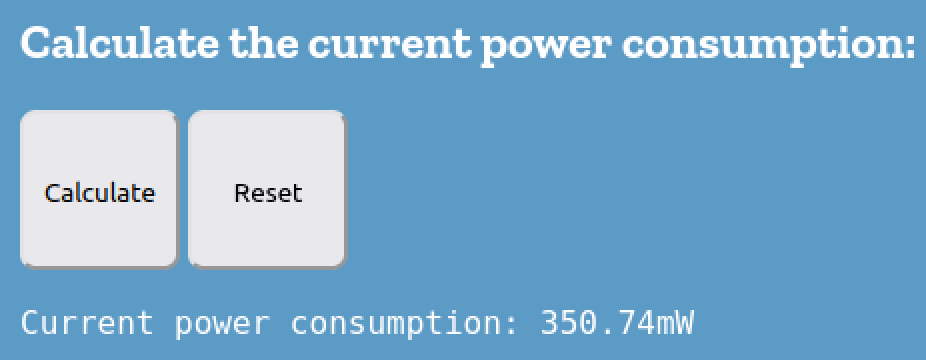
\includegraphics[scale=0.75]{images/addons/power-cons.png}
    \caption{Power off Extension front-end}
    \label{fig:t6v1fe}
\end{figure}

%\autoref{lst:t6calculus} shows that the calculus part of this extension is fine.

% \begin{lstlisting}[language=JavaScript, label=lst:t6calculus, caption=T6-v1 - Calculate Event]
% /* ... */
% calc_button.addEventListener('click', () => {
%           let sum = 0;
%           let plugs = 0;
  
%           window.API.getThings().then((res) => {
%             const jsonarray = res;  // Array of Things in JSON format
            
%             for (let n = 0; n < jsonarray.length; n++) {
%               let obj = jsonarray[n];
  
%               if (obj.properties.instantaneousPower !== undefined) {
%                 let uri = obj.id + "/properties/instantaneousPower";
  
%                 window.API.getJson(uri).then((res) => {
%                   let value = res.instantaneousPower;
%                   value = parseFloat(value);
%                   sum += value;
%                   plugs++;
%                   if(n === jsonarray.length-1) {
%                     pre.innerText = 
%                         `Current power consumption: ${(sum/plugs*1000).toFixed(2)}mW`;
%                   }
%                 })
%                 .catch( /* ... */ );  
%               }
%             }
%           });
%         });
%     /* ... */
% \end{lstlisting}

The portion of the extension that handles the reset leads to T6 (see \autoref{t6}) because it is implemented in such a way that once the Reset button is clicked, it  will temporarily alter the \texttt{instantaneousPower()} property, setting it to $0$. Of course, this extension will work only on smart device implementations that have the \texttt{instantaneousPower()} property not set as \texttt{readOnly}, as shown in \autoref{lst:t6reset}. Moreover, differently from the other \glspl{poc}, here the error is more on a conceptual level than on a programming level.

Hence, \autoref{lst:t6fix} shows how the reset event should be handled by just clearing the front-end.

\begin{lstlisting}[language=JavaScript, label=lst:t6reset, caption=T6-v1 - Reset Event]
/* ... */
reset_button.addEventListener('click', () => {
          window.API.getThings().then((res) => {
            const jsonarray = res;  // Array of Things in JSON format

            // Error: this loop resets the instantaneous power of the devices 
            for (let n = 0; n < jsonarray.length; n++) {
              let obj = jsonarray[n];
  
              if (obj.properties.instantaneousPower !== undefined &&
                obj.properties.instantaneousPower.readOnly !== true) {
                let uri = obj.id + "/properties/instantaneousPower";
  
                const body = {instantaneousPower: 0};
                window.API.putJson(uri, body)
                  .catch( /* ... */ );   
              }
            }
          });
          pre.innerText = "0mW";
        });
      }
    }
    /* ... */
\end{lstlisting}


\begin{lstlisting}[language=JavaScript, label=lst:t6fix, caption=T6-v1 - Fixed Reset]
/* ... */
reset_button.addEventListener('click', () => {
    // Fix: removed the wrong code lines
          pre.innerText = "";
        });
/* ... */
\end{lstlisting}



\subsection{T6-v2 - \texttt{plug-smart-adapter}}
\label{t62poc}

The \texttt{plug-smart-adapter} is an adapter add-on (see \autoref{adapter}). It integrates a virtual smart plug in the \gls{shg} and regularly stores its instantaneous power consumption data in a file. The adapter then reads all these data to calculate and show the average power consumption in the \gls{shg} dashboard among the device's properties. 

\begin{figure}[H]
    \centering
    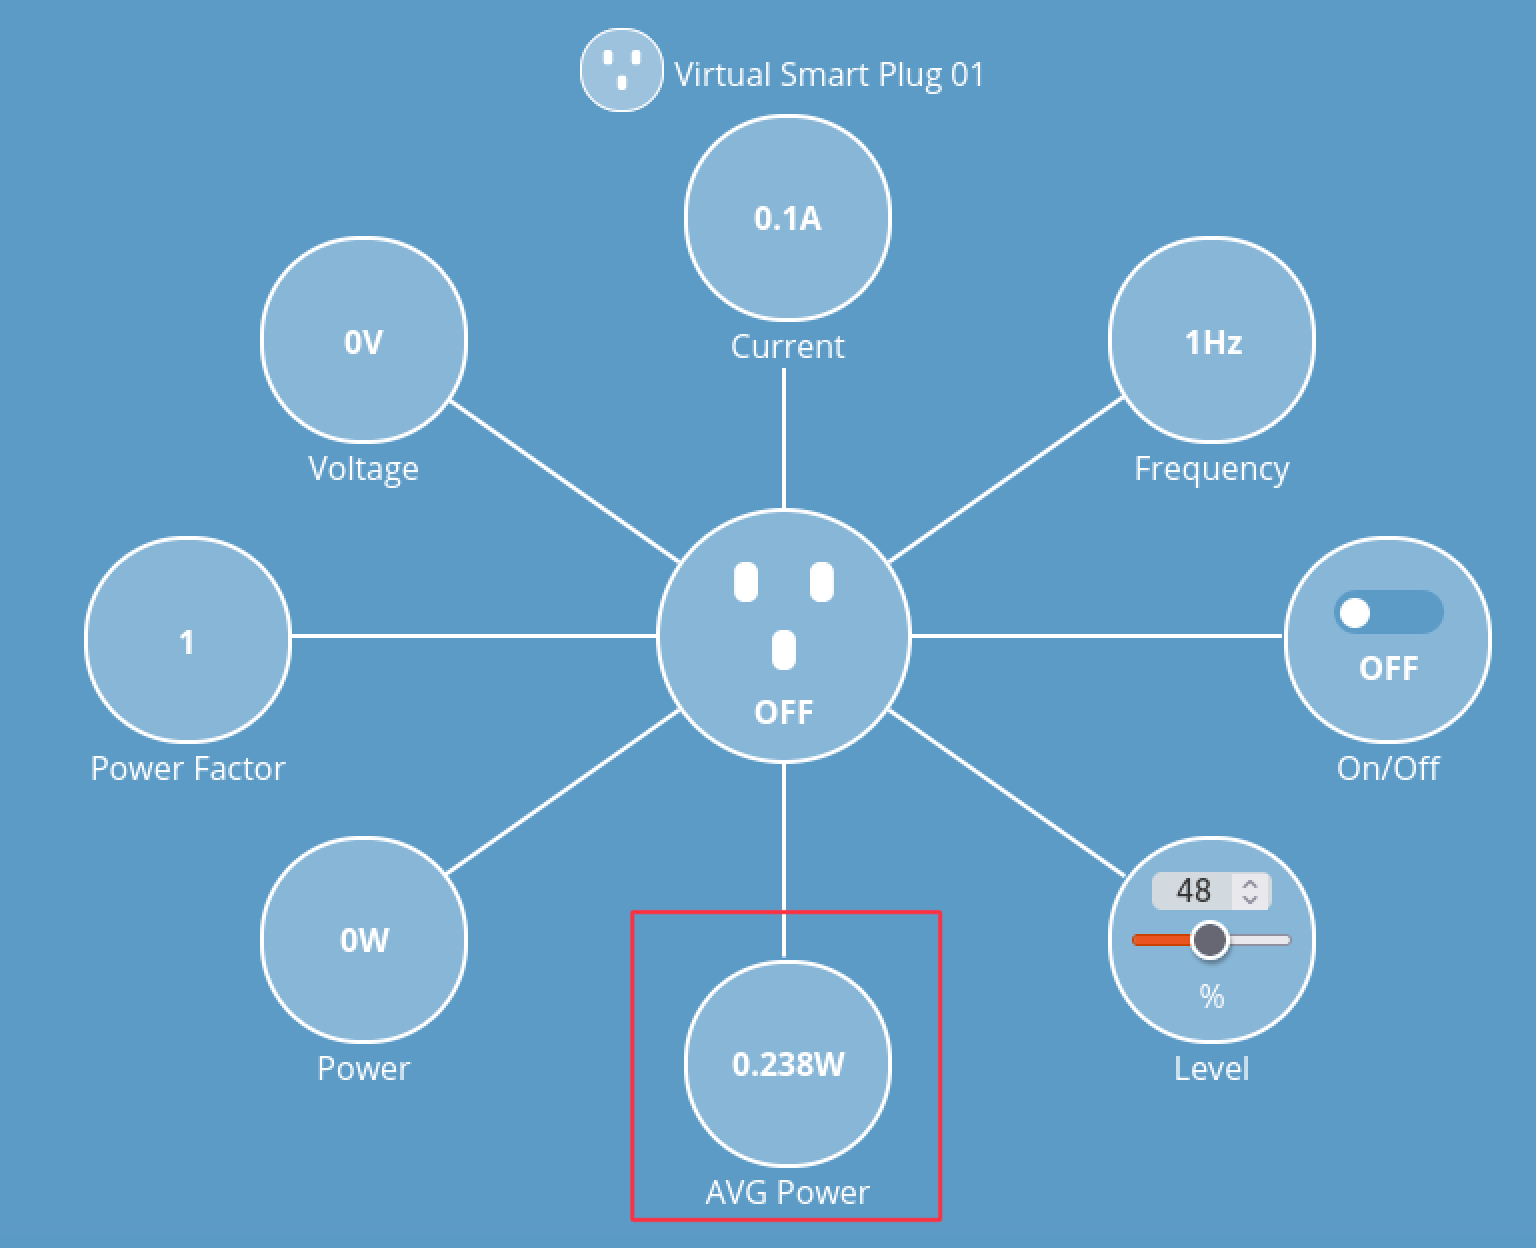
\includegraphics[scale=0.38]{images/addons/avg.png}
    \caption{Properties of a smart plug integrated through \texttt{plug-smart-adapter}}
\end{figure}

This adapter leads to T6 (see \autoref{t6}) because it has been implemented by using as a data path \path{~/.webthings/data/smart-plug-adapter}. The correct data path is \path{~/.webthings/data/plug-smart-adapter} instead. This error implies that if \texttt{smart-plug-adapter} exists and collects the same power consumption data in a file named as the one of \texttt{smart-plug-adapter}, the average power consumption output in the dashboard will be wrong for both the adapters. \autoref{lst:t6} shows the implementation details.

A possible fix of the adapter is shown in \autoref{lst:t6v2fix}.

\begin{lstlisting}[language=JavaScript, label=lst:t6, caption=T6-v2 - Plug Smart Adapter]
/* plug-smart-adapter */
 
 const baseDir = path.join(
    os.homedir(),
    ".webthings",
    "data",
    "smart-plug-adapter"  // Error: wrong data path
);

/* Property of a device */
class VirtualThingsProperty extends Property {
    constructor(device, name, descr, value, interval) {
      /* ... */
  
      if (/* ... */
         && this.name !== 'averagePowerConsumption') {
        /* ... */
      } else if (this.name === 'averagePowerConsumption') {
        this.interval = setInterval(() => {
          let sum = 0;
          const date = new Date();
          const year = /*...*/, month = /*...*/, day = /*...*/;
          let values = fs.readFileSync(
            path.join(baseDir, `powerValues-${year}${month}${day}.txt`), 'utf-8')
                .split('\n')
                .filter(value => value !== '');
          for (let i = 0; i < values.length; i++) {
            sum += parseFloat(values[i]);
          }
          this.value = (sum / values.length).toFixed(3);
          this.setCachedValue(this.value);
          this.device.notifyPropertyChanged(this);
        }, interval * 1000);
      } else if (this.name === 'instantaneousPower') {  
        this.interval = setInterval(() => {
          const date = new Date();
          const year = /*...*/, month = /*...*/, day = /*...*/;
          fs.appendFileSync(path.join(baseDir,
                    `powerValues-${year}${month}${day}.txt`),
            `${(this.value).toFixed(3)}\n`);
        }, interval*1000);    
      }
    }
}  
/* ... */
\end{lstlisting}


\begin{lstlisting}[language=JavaScript, label=lst:t6v2fix, caption=T6-v2 - Data Path Fix]
/* plug-smart-adapter */
 
 const baseDir = path.join(
    os.homedir(),
    ".webthings",
    "data",
    "plug-smart-adapter"  // Fix: correct data path
);
/* ... */
\end{lstlisting}


\subsection{T7 - \texttt{things-off-extension}}
\label{t7poc}

 This version of \texttt{things-off-extension}, like the one presented in \autoref{t5poc}, is an extension add-on (see \autoref{extension}). The add-on shows in the front-end of the Smart Home Gateway an OFF button. This button, when clicked, turns off every \glspl{web thing} in the Smart Home, i.e., every device controlled by the \gls{shg} having the \texttt{on()} property, with one second of delay from each other. \autoref{fig:t7fe} shows the extension in the front-end.

\begin{figure}[H]
    \centering
    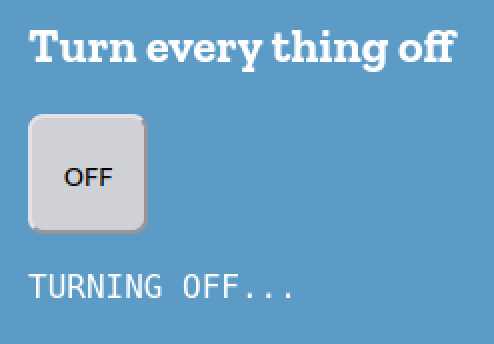
\includegraphics[scale=0.75]{images/addons/things-off.png}
    \caption{Things off Extension front-end}
    \label{fig:t7fe}
\end{figure}

However, the devices to turn off are stored inside an array. A loop iterates over each entry of the array of \glspl{web thing} --- that was filtered to just contain devices having the \texttt{on} property --- to turn them off. The problem is that the loop has a termination condition that is always true (see \autoref{lst:t7loop}). Hence, once reached the last \gls{web thing}, the add-on will keep turning it off. Therefore, the user will lose control over the last \gls{web thing} and will not be able anymore to turn and leave it on whenever it wants because it will be turned off again a few moments later resulting in T7 (see \autoref{t7}).

\autoref{lst:t7fix} shows the fixed \texttt{for} loop.

\begin{lstlisting}[language=JavaScript, label=lst:t7loop, caption=T7 - Turning off loop]
/* ... */
off_button.addEventListener('click', () => {
                pre.innerText = "TURNING OFF...";
                window.API.getThings().then((res) => {
                    const jsonarray = res  // Array of Things in JSON format
                        .filter(obj => obj.properties.on !== undefined);
        
                    let uri = "";
                    const body = {on: false};
                    for (let i = 0; jsonarray.length; i++) {  // Error: no termination condition
                        let obj = jsonarray[i];          
                        if (obj !== undefined) {
                            uri = obj.id + "/properties/on";
                        }
                        window.API.putJson(uri, body).catch(/* ... */);
                        sleep(1000);  // 1s delay
                    }
                }).catch(/* ... */);
            });

/* ... */
\end{lstlisting}


\begin{lstlisting}[language=JavaScript, label=lst:t7fix, caption=T7 - Fixed loop]
/* ... */
for (let i = 0; i < jsonarray.length; i++) {  // Fix: added the termination condition
    let obj = jsonarray[i];          
    if (obj !== undefined) {
        uri = obj.id + "/properties/on";
    }
    window.API.putJson(uri, body).catch(/* ... */);
    sleep(1000);  // 1s delay
}
}).catch(/* ... */);
/* ... */
\end{lstlisting}



\subsection{T8 - \texttt{smart-plug-adapter}}
\label{t8poc}

The \texttt{smart-plug-adapter} is a WebThings Gateway adapter add-on (see \autoref{adapter}). This adapter, every $15$ minutes, stores the instantaneous power consumption data of a virtual smart plug in a file. \autoref{fig:t8plug} shows a plug in the Smart Home Gateway dashboard.

\begin{figure}[H]
    \centering
    
\includegraphics[scale=0.75]{images/addons/simple-plug.png}
    \caption{Generic virtual plug in the dashboard}
    \label{fig:t8plug}
\end{figure}

This implementation of the adapter leads to T8 because in the \texttt{setInterval()} function, the argument that represents the delay is not $15$ minutes but $15$ seconds (see \autoref{lst:t8}). Therefore, assuming that the device which runs the \gls{shg} likely has a Solid State Drive (\gls{ssd}) memory \cite{micheloni2013inside} or a flash memory card whose life is affected by the number of writings \cite{li2019survey}, this implementation error will likely accelerate by $60$ times the breakdown of the device's memory and the memory fill time, other than consuming more resources and causing other related problems.

\autoref{lst:t8fix} shows how to easily fix the adapter.

\begin{lstlisting}[language=JavaScript, label=lst:t8, caption=T8 - \texttt{instantaneousPower} memorization]
/* ... */

/* Property of a device */
class VirtualThingsProperty extends Property {
    constructor(device, name, descr, value, interval) {
      /* ... */
  
     if (this.name === 'instantaneousPower') {  
        this.interval = setInterval(() => {
          const date = new Date();
          const year = /*...*/, month = /*...*/, day = /*...*/;
          fs.appendFileSync(path.join(baseDir, `powerValues-${year}${month}${day}.txt`),
            `${(this.value).toFixed(3)}\n`);
        }, 15 * 1000);  // Error: 15 seconds    
      }
    }
}
/* ... */
\end{lstlisting}


\begin{lstlisting}[language=JavaScript, label=lst:t8fix, caption=T8 - \texttt{setInterval()} fix]
/* ... */

/* Property of a device */
class VirtualThingsProperty extends Property {
    constructor(device, name, descr, value, interval) {
      /* ... */
  
     if (this.name === 'instantaneousPower') {  
        this.interval = setInterval(() => {
          const date = new Date();
          const year = /*...*/, month = /*...*/, day = /*...*/;
          fs.appendFileSync(
            path.join(baseDir, `powerValues-${year}${month}${day}.txt`),
            `${(this.value).toFixed(3)}\n`);
        }, 15 * 60 * 1000);  // Fix: 15 minutes
      }
    }
}
/* ... */
\end{lstlisting}



\section{Limitations}

\subsection{T9, T10, T11}
\label{t91011poc}

To briefly summarize which are the exploited threats, the related implementations and the security properties they break, this section groups them in \autoref{tab:pocs}.

\begin{table}[h!]
    \centering
    \begin{tabular}{| l | c | c | c |}
    \hline
    \textbf{Security Property} & \textbf{Threat} &  \textbf{Exploited} \\
    \hline
    Confidentiality & 
    \begin{tabular}{@{}c}T1 (\texttt{weather-adapter}) \\ T2 (\texttt{weather-adapter}) \end{tabular} &
    \begin{tabular}{@{}c}\checkmark \\ \checkmark \end{tabular} \\
    \hline
    Integrity &
    \begin{tabular}{@{}c}T3 (\texttt{lights-off-extension})\\ T4 (\texttt{smart-plugs-adapter}) \end{tabular} &
    \begin{tabular}{@{}c}\checkmark \\ \checkmark \end{tabular} \\
    \hline
    Availability &
    \begin{tabular}{@{}c}T5 (\texttt{things-off-extension}) \\ T6 (\texttt{power-cons-extension} \\ \texttt{plug-smart-adapter})\\ T7 (\texttt{things-off-extension})\\ T8 (\texttt{smart-plug-adapter}) \end{tabular} &
    \begin{tabular}{@{}c}\checkmark \\ \checkmark \\ \checkmark \\ \checkmark \end{tabular} \\
    \hline
    Authentication & 
    \begin{tabular}{@{}c}T9\end{tabular} & - \\  % mi urtava l'allineamento con le minacce sovrastanti
    \hline
    Authorization & T10 & - \\
    \hline
    Non-repudiation & T11 & - \\
    \hline
    \end{tabular}
    \caption{Exploited threats}
    \label{tab:pocs}
\end{table}

%Due to the nature of the WebThings Smart Home Gateway (\gls{shg}),
During the development of this thesis some attempts to implement Proofs of Concept (\glspl{poc}) exploiting T9, T10, and T11 were made.

T9 is about the authentication of an add-on. More precisely, an occurrence of this threat happens whenever an add-on successfully interacts with a system component pretending to be a different entity. T10, instead, is about authorization and it occurs when an add-on successfully accesses an authorization level higher than the one it should have.
Hence, having these two threats in mind, 
%my efforts were invested from the get-go to try to find a way to exploit both at once
I tried to exploit both at once. In WebThings the only category of add-on allowed to use the \gls{shg}'s \texttt{\glspl{api}} are the extensions (see \autoref{extension}). Therefore, an adapter add-on (see \autoref{adapter}) that successfully exploits these \texttt{\glspl{api}} would be an occurrence of both T9 and T10. However, the \gls{shg}'s authorization mechanisms are based on \texttt{JSON} Web Tokens (\textbf{\glspl{jwt}}), i.e., an open standard that defines a compact and self-contained way for securely transmitting information between parties as a \texttt{JSON} object \cite{rfc7519}. Each \texttt{\glspl{api}} call is authenticated through a \gls{jwt}, and I did not find a way to break this security mechanism to achieve the occurrences of T9 and T10 following this path. 
I also wondered about the authentication system of WebThings, and I tried to understand whether 
%there is an own property on the add-ons so that 
only the users that installed an add-on can use it. In this regard, the \gls{shg}, by default, has a multi-user capability, and each user authenticates itself through a username. Then, once inside the \gls{shg}, each user has access to the whole \gls{shg} add-ons and settings. Hence, each user has the same privileges and is not restricted to their personal user space and so do its add-ons.

T11, instead, is about non-repudiation and an occurrence of this threat implies that an add-on anonymously communicates with an attack target in such a way that there is no way to tell with certainty who were the parties involved in the communication. In this regard, I checked whether the \gls{shg} has some mechanisms to keep track of actions performed by its components (e.g., logging). However, WebThings, by default, just logs on file what is printed out on the console and does not specify to whose add-on that print belongs to. Thus, it becomes difficult to associate the actions performed within the platform with the agent who committed them.


\subsection{Devices}

It is important to point out that the \glspl{poc} have been developed and tested using virtual devices (i.e., weather stations, plugs and bulbs). However, this does not invalidate the outcomes of the study because what matters is not the device itself but the properties of that device and the way of interacting with it. In this sense, within the \gls{shg}, the properties of a virtual device are modeled like the ones of a physical device. For example, the \gls{shg} will model the \texttt{on} property of a physical light bulb in the same way as the \texttt{on} property of a virtual light bulb.



\section{Designing a new threat}
\label{t0appendix}

Since the beginning of this work, the importance of the add-ons' scope has been clear. It is
the set of resources an add-on is supposed to access legitimately (e.g., access tokens, configuration files, data folders, etc.). In this regard, the threat model used as a reference for this work is plenty of references to this scope.
As the study and development of the threats' \glspl{poc} proceeded, the lack of a mechanism that circumscribed the writing and reading space, or the permissions of a running add-on emerged. 
What has been said can become a problem when, for example, those who develop add-ons end up making two domains overlap on purpose, or by mistake (for example, in \autoref{t1poc}, \autoref{t2poc} and \autoref{t62poc}). Hence, during the development of this work a new threat, called \textbf{T0}, was designed.

\begin{itemize}
    \item \textbf{T0}: a plug-in scope could overlap the scope of another attack target.
\end{itemize}
This threat occurrence can lead to a very dangerous situation. More reasonably, the attack target can be another add-on. Indeed, if two add-ons share the same scope, it is possible to observe many of the threats presented in the threat model. For instance, an add-on could access, use, alter, and spread private data of the add-on which is sharing the scope with (T1, T2, T4). It could alter the state of other smart home devices (T3). It could delay the regular functionality of an attack target if it keeps using a resource within the scope needed also by other add-ons (T5). It could alter the regular functionality of an attack target (T6 or T7), and it could even damage the attack target by configuring wrong values.
If the add-on has access to the access token of another one could even interact with other entities pretending to be a different actor (T9), with a higher level than expected (T10) and even in an anonymous way (T11).

Although it seemed promising, during the study it was decided not to take it to the \gls{poc} development and validation stages, limiting the work to only developing \glspl{poc} for the threats already highlighted in the threat model. Therefore, a validation of this new proposal is left for future works.